\documentclass{beamer}
% \usepackage{beamerthemesplit}
\usetheme{Madrid}
% \usepackage{pstricks}
\usepackage{graphicx}
\usepackage{mdwlist}
\usepackage{lineno, hyperref}
\usepackage{stackrel}
\usepackage{changepage}

\usepackage{amssymb,latexsym,amsmath,amsthm,bbm}
\usepackage{hyperref}
\usepackage{tikz}
\usepackage[english]{babel}
\usepackage[latin1]{inputenc}
\usepackage[authoryear]{natbib}
\usepackage{multirow}
% \usepackage{enumitem}
\usepackage{verbatim}
\usepackage{alltt}
\newcommand{\btheta}{ \mbox{\boldmath $\theta$}}
\newcommand{\bmu}{ \mbox{\boldmath $\mu$}}
\newcommand{\balpha}{ \mbox{\boldmath $\alpha$}}
\newcommand{\bbeta}{ \mbox{\boldmath $\beta$}}
\newcommand{\bdelta}{ \mbox{\boldmath $\delta$}}
\newcommand{\blambda}{ \mbox{\boldmath $\lambda$}}
\newcommand{\bgamma}{ \mbox{\boldmath $\gamma$}}
\newcommand{\brho}{ \mbox{\boldmath $\rho$}}
\newcommand{\bpsi}{ \mbox{\boldmath $\psi$}}
\newcommand{\bepsilon}{ \mbox{\boldmath $\epsilon$}}
\newcommand{\bomega}{ \mbox{\boldmath $\omega$}}
\newcommand{\bOmega}{ \mbox{\boldmath $\Omega$}}
\newcommand{\bDelta}{ \mbox{\boldmath $\Delta$}}
\newcommand{\bSigma}{ \mbox{\boldmath $\Sigma$}}
\newcommand{\bPsi}{ \mbox{\boldmath $\Psi$}}
\newcommand{\bLambda}{ \mbox{\boldmath $\Lambda$}}

% \newcommand{\btheta}{\ensuremath{\mathbf{\theta}}}
% \newcommand{\bmu}{\ensuremath{\mathbf{\mu}}}
% \newcommand{\balpha}{\ensuremath{\mathbf{\alpha}}}
% \newcommand{\bbeta}{\ensuremath{\mathbf{\beta}}}
% \newcommand{\bdelta}{\ensuremath{\mathbf{\delta}}}
% \newcommand{\blambda}{\ensuremath{\mathbf{\lambda}}}
% \newcommand{\bgamma}{\ensuremath{\mathbf{\gamma}}}
% \newcommand{\brho}{\ensuremath{\mathbf{\rho}}}
% \newcommand{\bpsi}{\ensuremath{\mathbf{\psi}}}
% \newcommand{\bepsilon}{\ensuremath{\mathbf{\epsilon}}}
% \newcommand{\bomega}{\ensuremath{\mathbf{\omega}}}
% \newcommand{\bOmega}{\ensuremath{\mathbf{\Omega}}}
% \newcommand{\bDelta}{\ensuremath{\mathbf{\Delta}}}
% \newcommand{\bSigma}{\mbox{\boldmath $\Sigma$}}
% \newcommand{\bPsi}{\ensuremath{\mathbf{\Psi}}}
\newcommand{\bOne}{\ensuremath{\mathbf{1}}}
\newcommand{\bZero}{\ensuremath{\mathbf{0}}}

\newcommand{\omu}{\overline{\mu}}
\newcommand{\oSigma}{\overline{\Sigma}}
\newcommand{\Yt}{{\tilde Y}}
\newcommand{\alphahat}{\hat{\alpha}}

\newcommand{\bA}{\ensuremath{\mathbf{A}}}
\newcommand{\bB}{\ensuremath{\mathbf{B}}}
\newcommand{\bb}{\ensuremath{\mathbf{b}}}
\newcommand{\bfe}{\ensuremath{\mathbf{e}}}
\newcommand{\bG}{\ensuremath{\mathbf{G}}}
\newcommand{\bH}{\ensuremath{\mathbf{H}}}
\newcommand{\bh}{\ensuremath{\mathbf{h}}}
\newcommand{\bI}{\ensuremath{\mathbf{I}}}
\newcommand{\bL}{\ensuremath{\mathbf{L}}}
\newcommand{\bk}{\ensuremath{\mathbf{k}}}
\renewcommand{\bm}{\ensuremath{\mathbf{m}}}
\newcommand{\bo}{\ensuremath{\mathbf{o}}}
\newcommand{\bP}{\ensuremath{\mathbf{P}}}
\newcommand{\bR}{\ensuremath{\mathbf{R}}}
\newcommand{\br}{\ensuremath{\mathbf{r}}}
\newcommand{\bs}{\ensuremath{\mathbf{s}}}
\newcommand{\bt}{\ensuremath{\mathbf{t}}}
\newcommand{\bu}{\ensuremath{\mathbf{u}}}
\newcommand{\bV}{\ensuremath{\mathbf{V}}}
\newcommand{\bv}{\ensuremath{\mathbf{v}}}
\newcommand{\bW}{\ensuremath{\mathbf{W}}}
\newcommand{\bw}{\ensuremath{\mathbf{w}}}
\newcommand{\bX}{\ensuremath{\mathbf{X}}}
\newcommand{\bx}{\ensuremath{\mathbf{x}}}
\newcommand{\bY}{\ensuremath{\mathbf{Y}}}
\newcommand{\by}{\ensuremath{\mathbf{y}}}
\newcommand{\bZ}{\ensuremath{\mathbf{Z}}}
\newcommand{\bz}{\ensuremath{\mathbf{z}}}

\newcommand{\iid}{\stackrel{\mathrm{iid}}{\sim}}
\newcommand{\ind}{\stackrel{\mathrm{ind}}{\sim}}
\newcommand{\dd}{\; \text{d} }
\newcommand{\ddd}{\text{d} }
\newcommand{\indep}{\stackrel{\text{indep}}{\sim}}
\newcommand{\converged}{\stackrel{\mathrm{d}}{\rightarrow}}
\newcommand{\calR}{{\cal R}}
\newcommand{\calG}{{\cal G}}
\newcommand{\calD}{{\cal D}}
\newcommand{\calS}{{\cal S}}
\newcommand{\calB}{{\cal B}}
\newcommand{\calA}{{\cal A}}
\newcommand{\calT}{{\cal T}}
\newcommand{\calO}{{\cal O}}
\newcommand{\argmax}{{\mathop{\rm arg\, max}}}
\newcommand{\argmin}{{\mathop{\rm arg\, min}}}
\newcommand{\Frechet}{\mbox{Fr$\acute{\mbox{e}}$chet }}
\newcommand{\Matern}{\mbox{Mat$\acute{\mbox{e}}$rn }}
\newcommand{\ballunion}{B_a(\bs_1) \cup B_b(\bs_2) }
\newcommand{\skewt}{\mbox{skew-\emph{t}}}
\newcommand{\Skewt}{\mbox{Skew-\emph{t}}}
\newcommand{\tamarix}{\emph{Tamarix ramosissima}}
\newcommand{\hedysarum}{\emph{Hedysarum scoparium}}


\newcommand{\beq}{ \begin{equation}}
\newcommand{\eeq}{ \end{equation}}
\newcommand{\beqn}{ \begin{eqnarray}}
\newcommand{\eeqn}{ \end{eqnarray}}

\newcommand{\eref}[1]{(\ref{#1})}
\newcommand{\fref}[1]{Figure~\ref{#1}}
\newcommand{\tref}[1]{Table~\ref{#1}}
\newcommand{\sref}[1]{Section~\ref{#1}}
\newcommand{\aref}[1]{Appendix~\ref{#1}}
\newcommand{\cref}[1]{Chapter~\ref{#1}}

\newcommand*\patchAmsMathEnvironmentForLineno[1]{%
  \expandafter\let\csname old#1\expandafter\endcsname\csname #1\endcsname
  \expandafter\let\csname oldend#1\expandafter\endcsname\csname end#1\endcsname
  \renewenvironment{#1}%
     {\linenomath\csname old#1\endcsname}%
     {\csname oldend#1\endcsname\endlinenomath}}%
\newcommand*\patchBothAmsMathEnvironmentsForLineno[1]{%
  \patchAmsMathEnvironmentForLineno{#1}%
  \patchAmsMathEnvironmentForLineno{#1*}}%
\AtBeginDocument{%
\patchBothAmsMathEnvironmentsForLineno{equation}%
\patchBothAmsMathEnvironmentsForLineno{align}%
\patchBothAmsMathEnvironmentsForLineno{flalign}%
\patchBothAmsMathEnvironmentsForLineno{alignat}%
\patchBothAmsMathEnvironmentsForLineno{gather}%
\patchBothAmsMathEnvironmentsForLineno{multline}%
}

\newenvironment{response}{%
  \list{}{%
  	\setlength{\topmargin}{-1em}
  	\setlength{\leftmargin}{2em}
	\setlength{\rightmargin}{\leftmargin}
	\item[]
  }%
}{\vspace{1em}\endlist}


% \usepackage{cmbright}
\renewcommand*\familydefault{\sfdefault}
\usepackage[T1]{fontenc}

\graphicspath{{../Chapter-2/plots/}{../Chapter-3/plots/}{../Chapter-4/plots/}{./plots/}}

\definecolor{wp-red}{RGB}{204,0,0}
\definecolor{wp-gray}{RGB}{51,51,51}
\definecolor{reynolds-red}{RGB}{153,0,0}
\definecolor{pyroman-flame}{RGB}{209,81,34}
\definecolor{hunt-yellow}{RGB}{253,215,38}
\definecolor{genomic-green}{RGB}{125,140,31}
\definecolor{innovation-blue}{RGB}{66,126,147}
\definecolor{bio-indigo}{RGB}{65,86,161}

\setbeamercolor{structure}{fg=wp-red}
\setbeamercolor{title}{bg=white, fg=wp-red}  % changes color on title page
\setbeamerfont{title}{series=\bfseries, size=\huge}
\setbeamerfont{author}{series=\bfseries, size=\large}
\setbeamerfont{institute}{series=\mdseries, size=\large}

\setbeamercolor{frametitle}{bg=wp-red, fg=white}  % changes color at top of frame
\setbeamerfont{frametitle}{series=\bfseries}
\setbeamercolor{title in head/foot}{fg=white, bg=wp-red}  % changes color for title in footer
\setbeamerfont{title in head/foot}{series=\bfseries}
\setbeamercolor{author in head/foot}{fg=white,bg=wp-gray}  % changes color for author in footer
\setbeamerfont{author in head/foot}{series=\bfseries}

\title[Spatial methods for EVA] % (optional, use only with long paper titles)
{
  Spatial Methods for Modeling Extreme and Rare Events
}
\author[S. Morris]{Samuel A. Morris}
\institute[]{North Carolina State University}
\date[]{August 22, 2016}

\begin{document}

\begin{frame}\frametitle{\ }
\begin{center}
  \maketitle
\end{center}
\end{frame}


\begin{frame}{Outline}
\begin{itemize} \setlength{\itemsep}{1em}
	\item Brief overview of theory for extremes
	\item Three principal contributions:
	\begin{enumerate}[1.]\setlength{\itemsep}{0.5em}
		\item A spatio-temporal model with flexible tails, asymptotic spatial dependence, and computation on the order of Gaussian models for large space-time datasets (Biometrics)
		\item Modeling spatial rare binary events with a max-stable extension to the GEV link function (JABES)
		\item Empirical basis functions to explore and model extremal spatial dependence (AOAS)
	\end{enumerate}
\end{itemize}	
\end{frame}

\begin{frame}{Motivation}
  \begin{itemize} \setlength{\itemsep}{1em}
    \item Average behavior is important to understand, but it does not paint the whole picture
    \begin{itemize}
      \item e.g. When constructing river levees, engineers need to be able to estimate a 100-year or 1000-year flood levels
      \item e.g. Probability of ambient air pollution exceeding a certain threshold level
    \end{itemize}
    \item Estimating the probability of rare events is challenging because these events are, by definition, rare
    \item Spatial extremes is promising because it borrows information across space
    \item Spatial extremes is also useful for estimating probability of extremes at sites without data
  \end{itemize}
\end{frame}

 \begin{frame}{Motivation}
   \centering
   \begin{figure}
     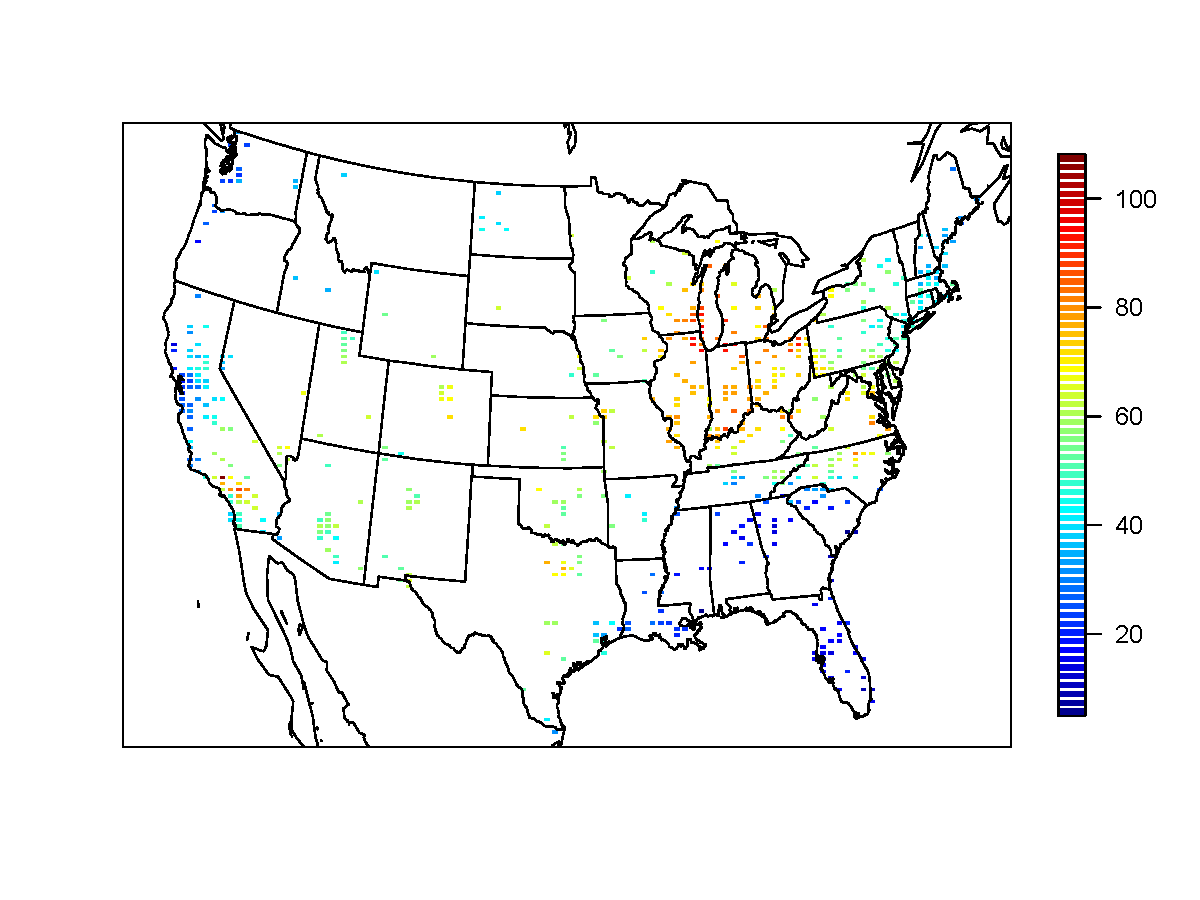
\includegraphics[width=\linewidth, trim=0 1in 0 1in ]{ozone-10jul-us}
     \caption{Max 8-hour ozone measurements on July 10, 2005}
    \end{figure}
 \end{frame}

 \begin{frame}{Motivation}
 \begin{adjustwidth}{1em}{0em}
   Ozone compliance for Clean Air Act (EPA) \vspace{1em}
   \begin{itemize} \setlength{\itemsep}{1em}
     \item Annual fourth-highest daily maximum 8-hour concentration, averaged over 3 years, not to exceed 75 ppb
     \item Annual fourth-highest is the 99th percentile for the year
     \item Common objectives are \vspace{0.5em}
     \begin{itemize} \setlength{\itemsep}{0.5em}
       \item To interpolate to unmonitored sites
       \item Detect changes in extremes over time
       \item Study meteorological conditions that lead to extreme events
     \end{itemize}
   \end{itemize}
 \end{adjustwidth}
 \end{frame}

 \begin{frame}{Defining extremes}
 \begin{columns}[c]
 \column{.45 \linewidth}
   \begin{itemize} \setlength{\itemsep}{1em}
     \item Key in extreme value analysis is to define extremes
     \item Typically done in one of two ways
     \begin{itemize}
       \item Block maxima (red dots)
       \item Values over threshold considered extreme
     \end{itemize}
   \end{itemize}

   \column{.55\linewidth}
   \begin{figure}
     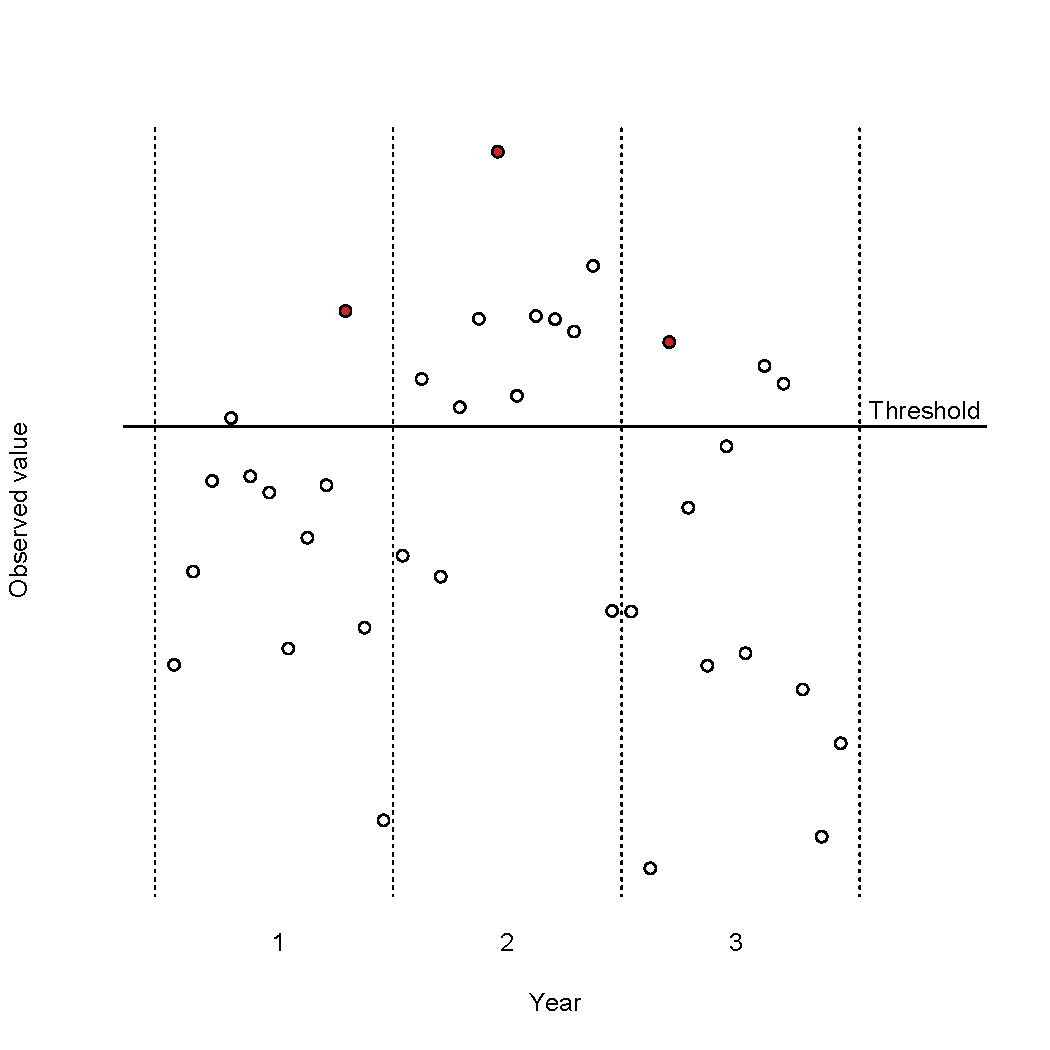
\includegraphics[width=1\linewidth, trim=0 0.5in 0 1in]{./plots/define_extreme.pdf}
     \caption{Hypothetical monthly data}
     \end{figure}
 \end{columns}
 \end{frame}

 \begin{frame}{Non-spatial analysis: Block maxima}
 \begin{adjustwidth}{1em}{0em}
   Fisher-Tippett-Gnedenko theorem \vspace{1em}
   \begin{itemize} \setlength{\itemsep}{1em}
     \item Let $X_1, \ldots, X_n$ be i.i.d.
     \item Consider the block maximum $M_n = \max(X_1, \ldots, X_n)$
     \item If there exist normalizing sequences $a_n > 0$ and $b_n \in \calR$ such that
     \begin{align*}
       \frac{ M_n - b_n }{ a_n } \converged G(z)
     \end{align*}
     then $G(z)$ follows a generalized extreme value distribution (GEV) (Gnedenko, 1943)
     \item This motivates the use of the GEV for block maximum data
   \end{itemize}
 \end{adjustwidth}
 \end{frame}

 \begin{frame}{Non-spatial analysis: Block maxima}
   \begin{itemize} \setlength{\itemsep}{1em}
     \item GEV distribution
     \begin{align*}
       G(y) = \Pr(Y < y) = \left\{  \begin{array}{ll}
         \exp\left\{ -\left[ 1 + \xi \left( \frac{ y - \mu }{ \sigma } \right) \right]^{ -1 / \xi} \right\} & \quad \xi \neq 0 \\[0.5em]
         \exp \left\{ -\exp \left( - \frac{ y - \mu }{ \sigma} \right) \right\} & \quad \xi = 0
       \end{array}\right.
     \end{align*}
     where
     \begin{itemize} \setlength{\itemsep}{0.25em}
       \item $\mu \in \calR$ is a location parameter
       \item $\sigma > 0$ is a scale parameter
       \item $\xi \in \calR$ is a shape parameter
       \begin{itemize}
         \item Unbounded above if $\xi \ge 0$
         \item Bounded above by $(\mu - \sigma) / \xi$ when $\xi < 0$
       \end{itemize}
     \end{itemize}
     \item Challenges:
     \begin{itemize}
       \item Lose information by only considering maximum in a block
       \item Underlying data may not be i.i.d.
     \end{itemize}
   \end{itemize}
 \end{frame}

 \begin{frame}{Non-spatial analysis: Peaks over threshold}
 \begin{adjustwidth}{1em}{0em}
   Pickands-Balkema-de Haan theorem \vspace{1em}
   \begin{itemize} \setlength{\itemsep}{1em}
     \item Let $X_1, \ldots, X_n \iid F$
     \item If there exist normalizing sequences $a_T > 0$ and $b_T \in \calR$ such that for any $x \ge 0$, as $T \rightarrow \infty$
     \begin{align*}
       \Pr\left(\frac{X - b_T}{a_T} > x \mid X > T\right) \converged H(x),
     \end{align*}
     where $T$ is a thresholding value, then $H(x)$ follows a generalized Pareto distribution (GPD) (Balkema and de Haan, 1974)
   \end{itemize}
 \end{adjustwidth}
 \end{frame}

 \begin{frame}{Non-spatial analysis: Peaks over threshold}
 \begin{adjustwidth}{1em}{0em}
   Select a threshold, $T$, and use the GPD to model the exceedances
   \begin{align*}
     H(y) = P(Y < y) = \left\{ \begin{array}{ll}
       1 - \left[1 - \xi \left( \frac{ y - T }{ \sigma } \right) \right]^{-1 / \xi} & \quad \xi \neq 0 \\[0.5em]
       1 - \exp \left\{ \frac{ y - T }{ \sigma} \right\} & \quad \xi = 0
     \end{array}\right.
   \end{align*}
   where
   \begin{itemize} \setlength{\itemsep}{0.25em}
     \item $\sigma > 0$ is a scale parameter
     \item $\xi \in \calR$ is a shape parameter
     \begin{itemize}
       \item Unbounded above if $\xi \ge 0$
       \item Bounded above by $(T - \sigma) / \xi$ when $\xi < 0$
     \end{itemize}
   \end{itemize}
 \end{adjustwidth}
 \end{frame}

 \begin{frame}{Non-spatial analysis: Peaks over threshold}
   \begin{itemize} \setlength{\itemsep}{1em}
     \item The GPD is related to GEV distribution through
     \begin{align*}
       H(y) = 1 + \log[G(y)], \quad y \ge T
     \end{align*}
     \item Challenges: \vspace{0.5em}
     \begin{itemize} \setlength{\itemsep}{0.5em}
       \item Sensitive to threshold selection
       \item Temporal dependence between observations (e.g. flood levels don't dissipate overnight)
     \end{itemize}
   \end{itemize}
 \end{frame}

 \begin{frame}{Max-stable processes for spatial data}
   \begin{itemize} \setlength{\itemsep}{1em}
     \item Consider i.i.d. spatial processes $x_j(\bs)$, $j = 1, \ldots, J$
     \item Let $M_J(\bs) = \bigvee_{j=1}^J x_j(\bs_i)$ be the block maximum at site $\bs$
     \item If there exists normalizing sequences $a_J(\bs)$ and $b_J(\bs)$ such that for all sites, $\bs_i, i = 1, \ldots, d$,
     \begin{align*}
       \frac{M_J(\bs) - b_J(\bs)}{a_J(\bs)} \converged G(\bs)
     \end{align*}
     then $G(\bs)$ is a max-stable process (Smith, 1990)
     \item Therefore, max-stable processes are the standard model for block maxima
   \end{itemize}
 \end{frame}

 \begin{frame}{Multivariate representations}
   \begin{itemize} \setlength{\itemsep}{1em}
     \item Marginally at each site, observations follow a GEV distribution
     \item For a finite collection of sites the representation for the multivariate GEV (mGEV) is
     \begin{align*}
       \Pr(\bZ \le \bz)  &= G^*(\bz) = \exp[-V(\bz)]\\
             V(\bz)    &= d \int_{\Delta_d} \bigvee_{i = 1}^d \frac{w_i}{z_i} H(\ddd w)
     \end{align*}
     where
     \begin{itemize} \setlength{\itemsep}{0.25em}
       \item $V(\bz)$ is called the exponent measure
       \item $\Delta_d = \{ \bw \in \calR^d_+ \mid w_1 + \cdots + w_d = 1\}$
       \item $H$ is a probability measure on $\Delta_d$
       \item $\int_{\Delta_d}w_i H(\ddd w) = 1 / d$ for $i = 1, \ldots, d$
     \end{itemize}
   \end{itemize}
 \end{frame}

 \begin{frame}{Multivariate GEV challenges}
   \begin{itemize} \setlength{\itemsep}{1em}
     \item Only a few closed-form expressions for $V(\bz)$ exist
     \item Two common forms for $V(\bz)$
     \begin{itemize}
       \item Symmetric logistic (Gumbel, 1960)
       \begin{align*}
         V(\bz) = \left[\sum_{i = 1}^n \left( \frac{ 1 }{ z_i } \right)^{1/\alpha}\right]^\alpha
       \end{align*}
       \item Asymmetric logistic (Coles and Tawn, 1991)
       \begin{align*}
         V(\bz) = \sum_{l = 1}^L \left[\sum_{i = 1}^n \left(\frac{w_{il}}{z_i} \right)^{1 / \alpha_l} \right]^{\alpha_l}
       \end{align*}
       where $w_{il} \in [0, 1]$ and $\sum_{l = 1}^L w_{il} = 1$
     \end{itemize}
   \end{itemize}
 \end{frame}

 %\begin{frame}{Multivariate peaks over threshold}
 %  \begin{itemize} \setlength{\itemsep}{1em}
 %    \item Few existing methods
 %    \item Often use max-stable methods due to the relationship between GEV and GPD
 %    \item Joint distribution function given by Falk et al. (2011)
 %    \begin{align*}
 %      H(\bz) = 1 - V(\bz)
 %    \end{align*}
 %    where $V(\bz)$ is defined as in the GEV
 %  \end{itemize}
 %\end{frame}

 \begin{frame}{Extremal dependence: $\chi$ statistic}
   \begin{itemize} \setlength{\itemsep}{1em}
     \item Correlation is the most common measure of dependence
     \begin{itemize}
       \item Focuses on the center and not tails
       \item This makes it irrelevant for extreme value analysis
     \end{itemize}
     \item Extreme value analysis focuses on the $\chi$ statistic (Coles et al., 1999), a measure of extremal dependence given by
     \begin{align*}
       \chi(h) = \lim_{c \rightarrow \infty}\Pr[Y(\bs) > c \mid Y(\bt) > c]
     \end{align*}
     where $h = ||\bs - \bt||$
     \item If $ \chi(h) = 0$, then observations are asymptotically independent at distance $h$
   \end{itemize}
 \end{frame}

 \begin{frame}{Existing challenges}
   \begin{itemize} \setlength{\itemsep}{1em}
     \item Multivariate max-stable models have nice features, but they are
     \begin{itemize}
       \item Computationally challenging (e.g,  the asymmetric logistic has $2^{n-1}(n + 2) - (2n + 1)$ free parameters)
       \item Joint density only available in low dimensions
     \end{itemize}
     \item Some recent approaches
     \begin{itemize}
       \item Bayesian hierarchical model (Reich and Shaby, 2012)
       \item Pairwise likelihood approach (Huser and Davison, 2014)
     \end{itemize}
     \item Many opportunities to explore new methods
   \end{itemize}
 \end{frame}


 \begin{frame}\frametitle{Back to a Gaussian process model}
 	\begin{itemize}\setlength\itemsep{\fill}
 	\item The max-stable process is an elegant approach, but does that mean it's the right model?
 	\item In reality, it is only an approximation
 	\item There are less complicated approximations
 	\item For example, we could model daily data as a Gaussian process (GP)
 	\item If the goal is spatial interpolation, perhaps this is competitive
 	\end{itemize}
 \end{frame}


 \begin{frame}\frametitle{GP - asymptotic independence}
 	\begin{itemize}\setlength\itemsep{\fill}
 	\item A GP leads to simple interpretation and computing, but asymptotic independence
 	\item If $Y(\bs_1)$ and $Y(\bs_2)$ are bivariate normal then $\chi(\bs_1,\bs_2)=0$, i.e., asymptotic independence
 	\item This suggests Kriging will not capture extremes
 	\item But so much is known for the Gaussian case: nonstationarity, multivariate, numerical approximations, \ldots
 	\item Rather than toss it out, can we patch it up?
 	\end{itemize}
 \end{frame}


\begin{frame}\frametitle{Spatial \skewt{} process}
A spatial \skewt{} process (Azzalini and Capitanio, 2014)  resembles a GP but exhibits asymptotic dependence
	\begin{eqnarray}
	 	Y_t(\bs) &=& \bX(\bs)^\top\bbeta +\lambda\sigma_t|z_t| + \sigma_tv_t(\bs)\nonumber\\
	 	z_t &\sim& \mbox{Normal}(0,1)\nonumber\\
	 	\sigma_t^2&\sim& \mbox{InvGamma}(a/2,b/2)\nonumber\\
	 	v_t&\sim& \mbox{Spatial GP}\nonumber
 	\end{eqnarray}
 	\begin{itemize}\setlength\itemsep{\fill}
	 	\item Location: $\bX(\bs)^\top\bbeta$
	 	\item Scale: $b>0$
	 	\item Skewness: $\lambda\in{\cal R}$
	 	\item Degrees of freedom: $a>0$
	\end{itemize}
\end{frame}



 \begin{frame}\frametitle{Good properties}
 	\begin{itemize}\setlength\itemsep{\fill}
 	\item Flexible $t$ marginal distribution with four parameters including the degrees of freedom which allows for heavy tails ($a=1$ gives a Cauchy)
 	\item Computation on the order of a GP; the only extra steps are $z_t$ and $\sigma_t$ which have conjugate full conditionals
 	\item Asymptotic dependence: $\chi(\bs_1,\bs_2)>0$ for all $\bs_1$ and $\bs_2$
 	\end{itemize}
 \end{frame}

 \begin{frame}\frametitle{Bad properties and remedies}
 	\begin{itemize}\setlength\itemsep{1em}
 	\item Modeling all the data (bulk and extreme) can lead to poor tail probability estimates if the model is misspecified
 	\item Long-range dependence: $\chi(\bs_1,\bs_2)>0$ for all $\bs_1$ and $\bs_2$ even if $\bs_1$ and $\bs_2$ are far apart
 	\item This occurs because all sites share $z_t$ and $\sigma_t$
 	\item Remedies:
 	\begin{itemize}
 	\item We use a censored likelihood to focus on the tails
 	\item We propose a local \skewt{} process
 	\end{itemize}
 	\end{itemize}
 \end{frame}

 \begin{frame}\frametitle{Censored likelihood}
 	\begin{itemize}\setlength\itemsep{\fill}
 	\item Censored likelihood: We censor the data
 	$${\tilde Y}_t(\bs) =\left\{\begin{array}{ll}
 	T & \text{for } Y_t(\bs)\le T\\
 	Y_t(\bs) & \text{for } Y_t(\bs)>T
 	\end{array}\right.$$
 	\item Censoring is handled using standard Bayesian imputation methods
 	\item The threshold $T$ is chosen by cross-validation
 	\item If $T$ is moderately extreme in the distribution (e.g. $q(0.75)$), set $\lambda = 0$
 	\end{itemize}
 \end{frame}

 \begin{frame}\frametitle{Local \skewt{} process}
 	\begin{itemize}\setlength\itemsep{\fill}
 	\item Let the knots $\bv_{t1},...,\bv_{tK}$ follow a homogeneous Poisson process over the domain of interest (in practice we fix $K$)
 	\item Associated with each is
 	\begin{itemize}
 		\item $z_{tk}\sim\mbox{Normal}(0,1)$
 		\item $\sigma_{tk}^2\sim\mbox{InvGamma}(a/2,b/2)$
 	\end{itemize}
 	\item The knots partition the domain if we assign location $\bs$ to subregion $k=\argmin_{l}||\bs-\bv_{tl}||$
 	\item If $\bs$ is in subregion $k$ then $$Y_t(\bs) = \bX(\bs)^T\bbeta +\lambda\sigma_{tk}|z_{tk}| + \sigma_{tk}v_t(\bs)\nonumber$$
 	\item The marginal distribution remains a $t$, but partitioning breaks long-range spatial dependence
 	\end{itemize}
 \end{frame}

 \begin{frame}\frametitle{$\chi$-statistic by $h=||\bs_1-\bs_2||$}
 	\begin{center}
 		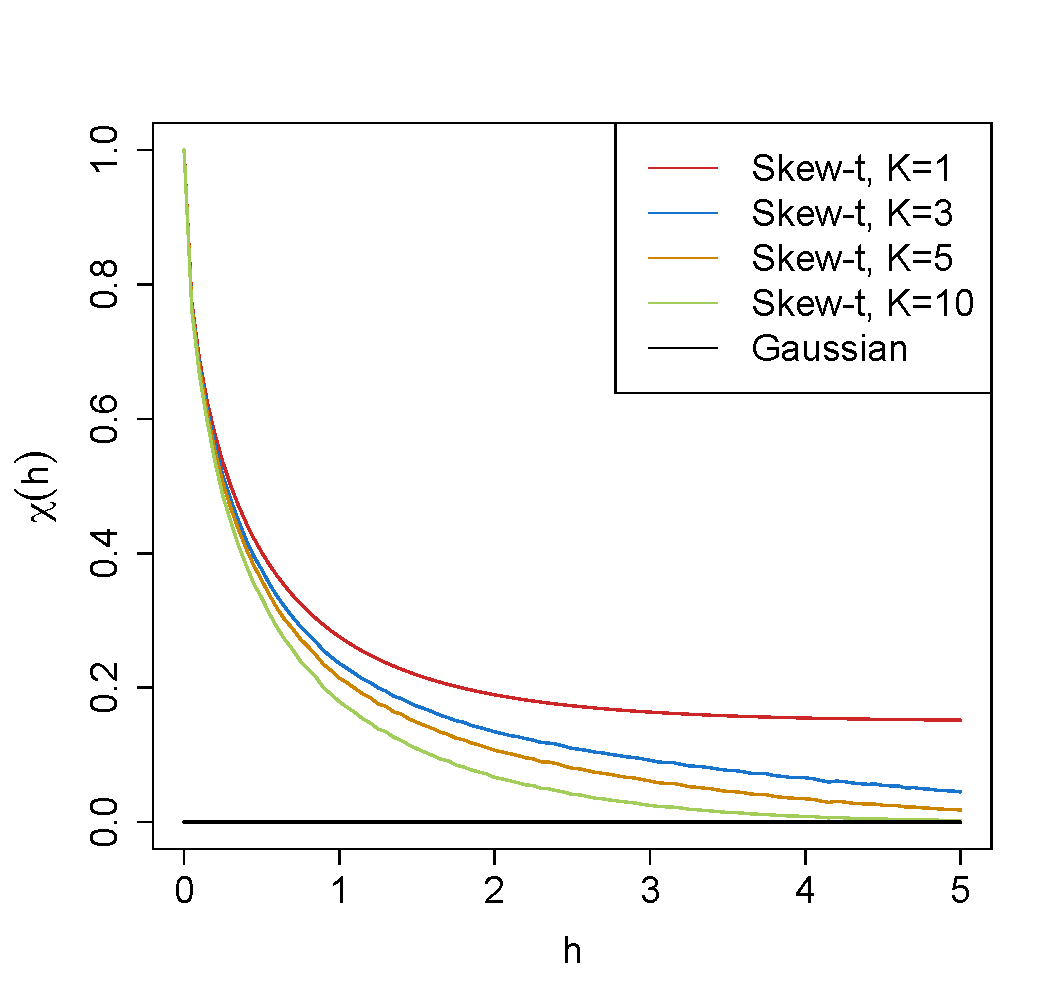
\includegraphics[height=0.8\textheight]{plots/chi-h}
 	\end{center}
 \end{frame}

 \begin{frame}\frametitle{Temporal dependence}
 	\begin{itemize}\setlength\itemsep{1em}
 	\item It may not be reasonable to assume that observations are temporally independent (e.g. flooding, high temperatures)
 	\item Temporal dependence is handled through the $z_{tk}$, $\sigma_{tk}$ and $\bv_{tl}$
 	\item Method:
 	\begin{itemize}\setlength\itemsep{0.5em}
 	\item Use a copula to transform parameters to \emph{nice} space (i.e. $\mathcal{R}$)
 	\item AR(1) structure imposed on parameters in transformed space
 	\item Transform back to original parameter space to preserve \skewt{}
 	\end{itemize}
 	\end{itemize}
 \end{frame}


\begin{frame}\frametitle{Results of a simulation study}
In terms of Brier scores for spatial prediction:\vspace{1em}
\begin{itemize}\setlength\itemsep{1em}
	\item Data generated as a GP:
	\begin{itemize}
	 	\item \skewt{} is close to GP
	 	\item max-stable is 15\% -- 30\% worse than GP
	\end{itemize}
	\item Data generated as a \skewt{} with multiple partitions:
	\begin{itemize}
		\item \skewt{} is 15\% better than GP
	 	\item max-stable is 30\% worse than GP
	\end{itemize}
	\item Data generated as asymmetric logistic (max-stable):
	\begin{itemize}
		\item \skewt{} is close to GP
		\item max-stable performs 10\% better than GP
	\end{itemize}
 	\item Data generated as Brown-Resnick (max-stable):
 	\begin{itemize}
		\item \skewt{} performs 40\% -- 60\% better than GP
 		\item max-stable performs 40\% -- 60\% better than GP
 	\end{itemize}
\end{itemize}
\end{frame}


 \begin{frame}\frametitle{Application to ozone}
 	\begin{itemize}\setlength\itemsep{\fill}
 	\item The USEPA has an extensive network of ozone monitors throughout the US
 	\item We will analyze ozone for 31 days in July, 2005 at $n=1,089$ stations
 	\item Currently the EPA regulates the annual 99$^{th}$ percentile
 	\item Our objective is to map the probability of an extreme ozone event
 	\end{itemize}
 \end{frame}

 \begin{frame}\frametitle{Ozone on July 10}
 	\begin{center}
 		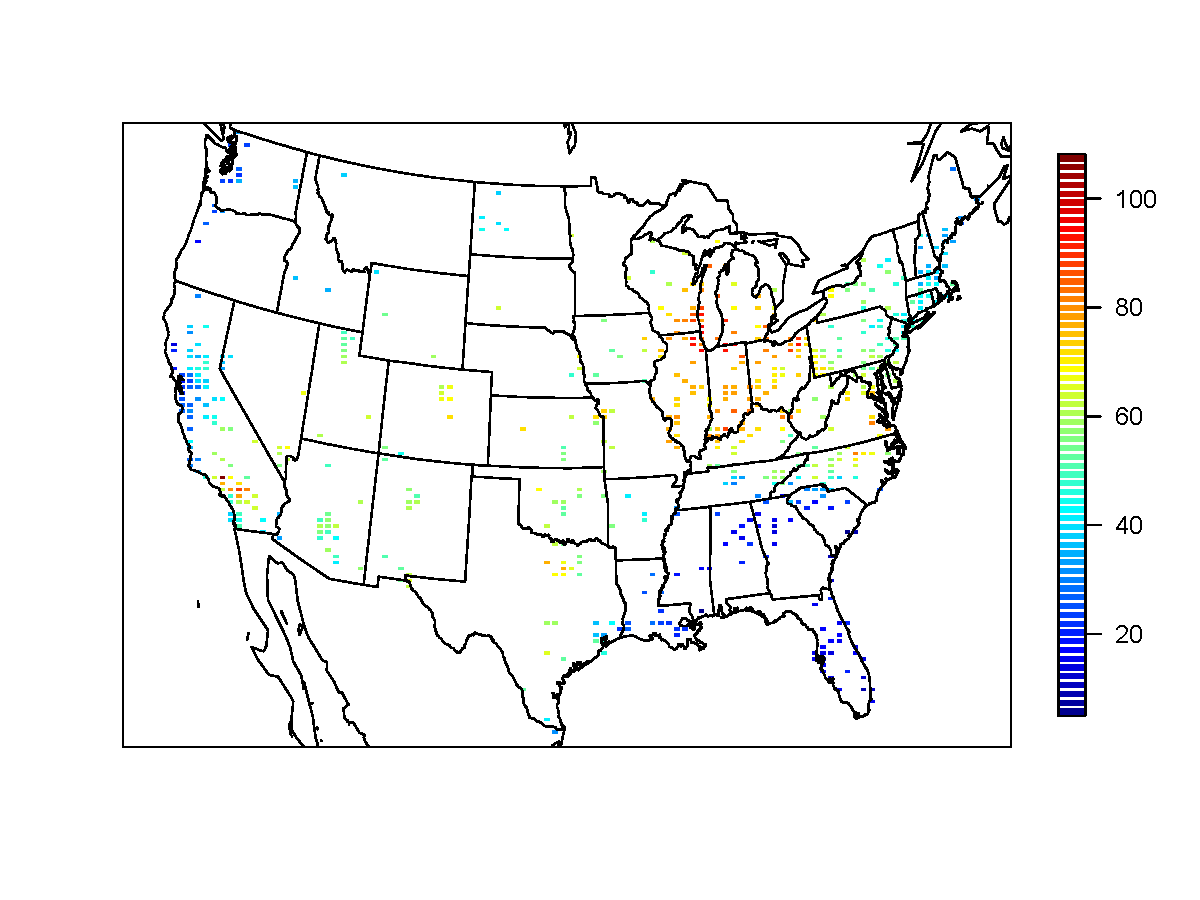
\includegraphics[width=1.2\textheight]{ozone-10jul-us}
 	\end{center}
 \end{frame}

 \begin{frame}\frametitle{Q-Q plots}
 	\begin{center}
 		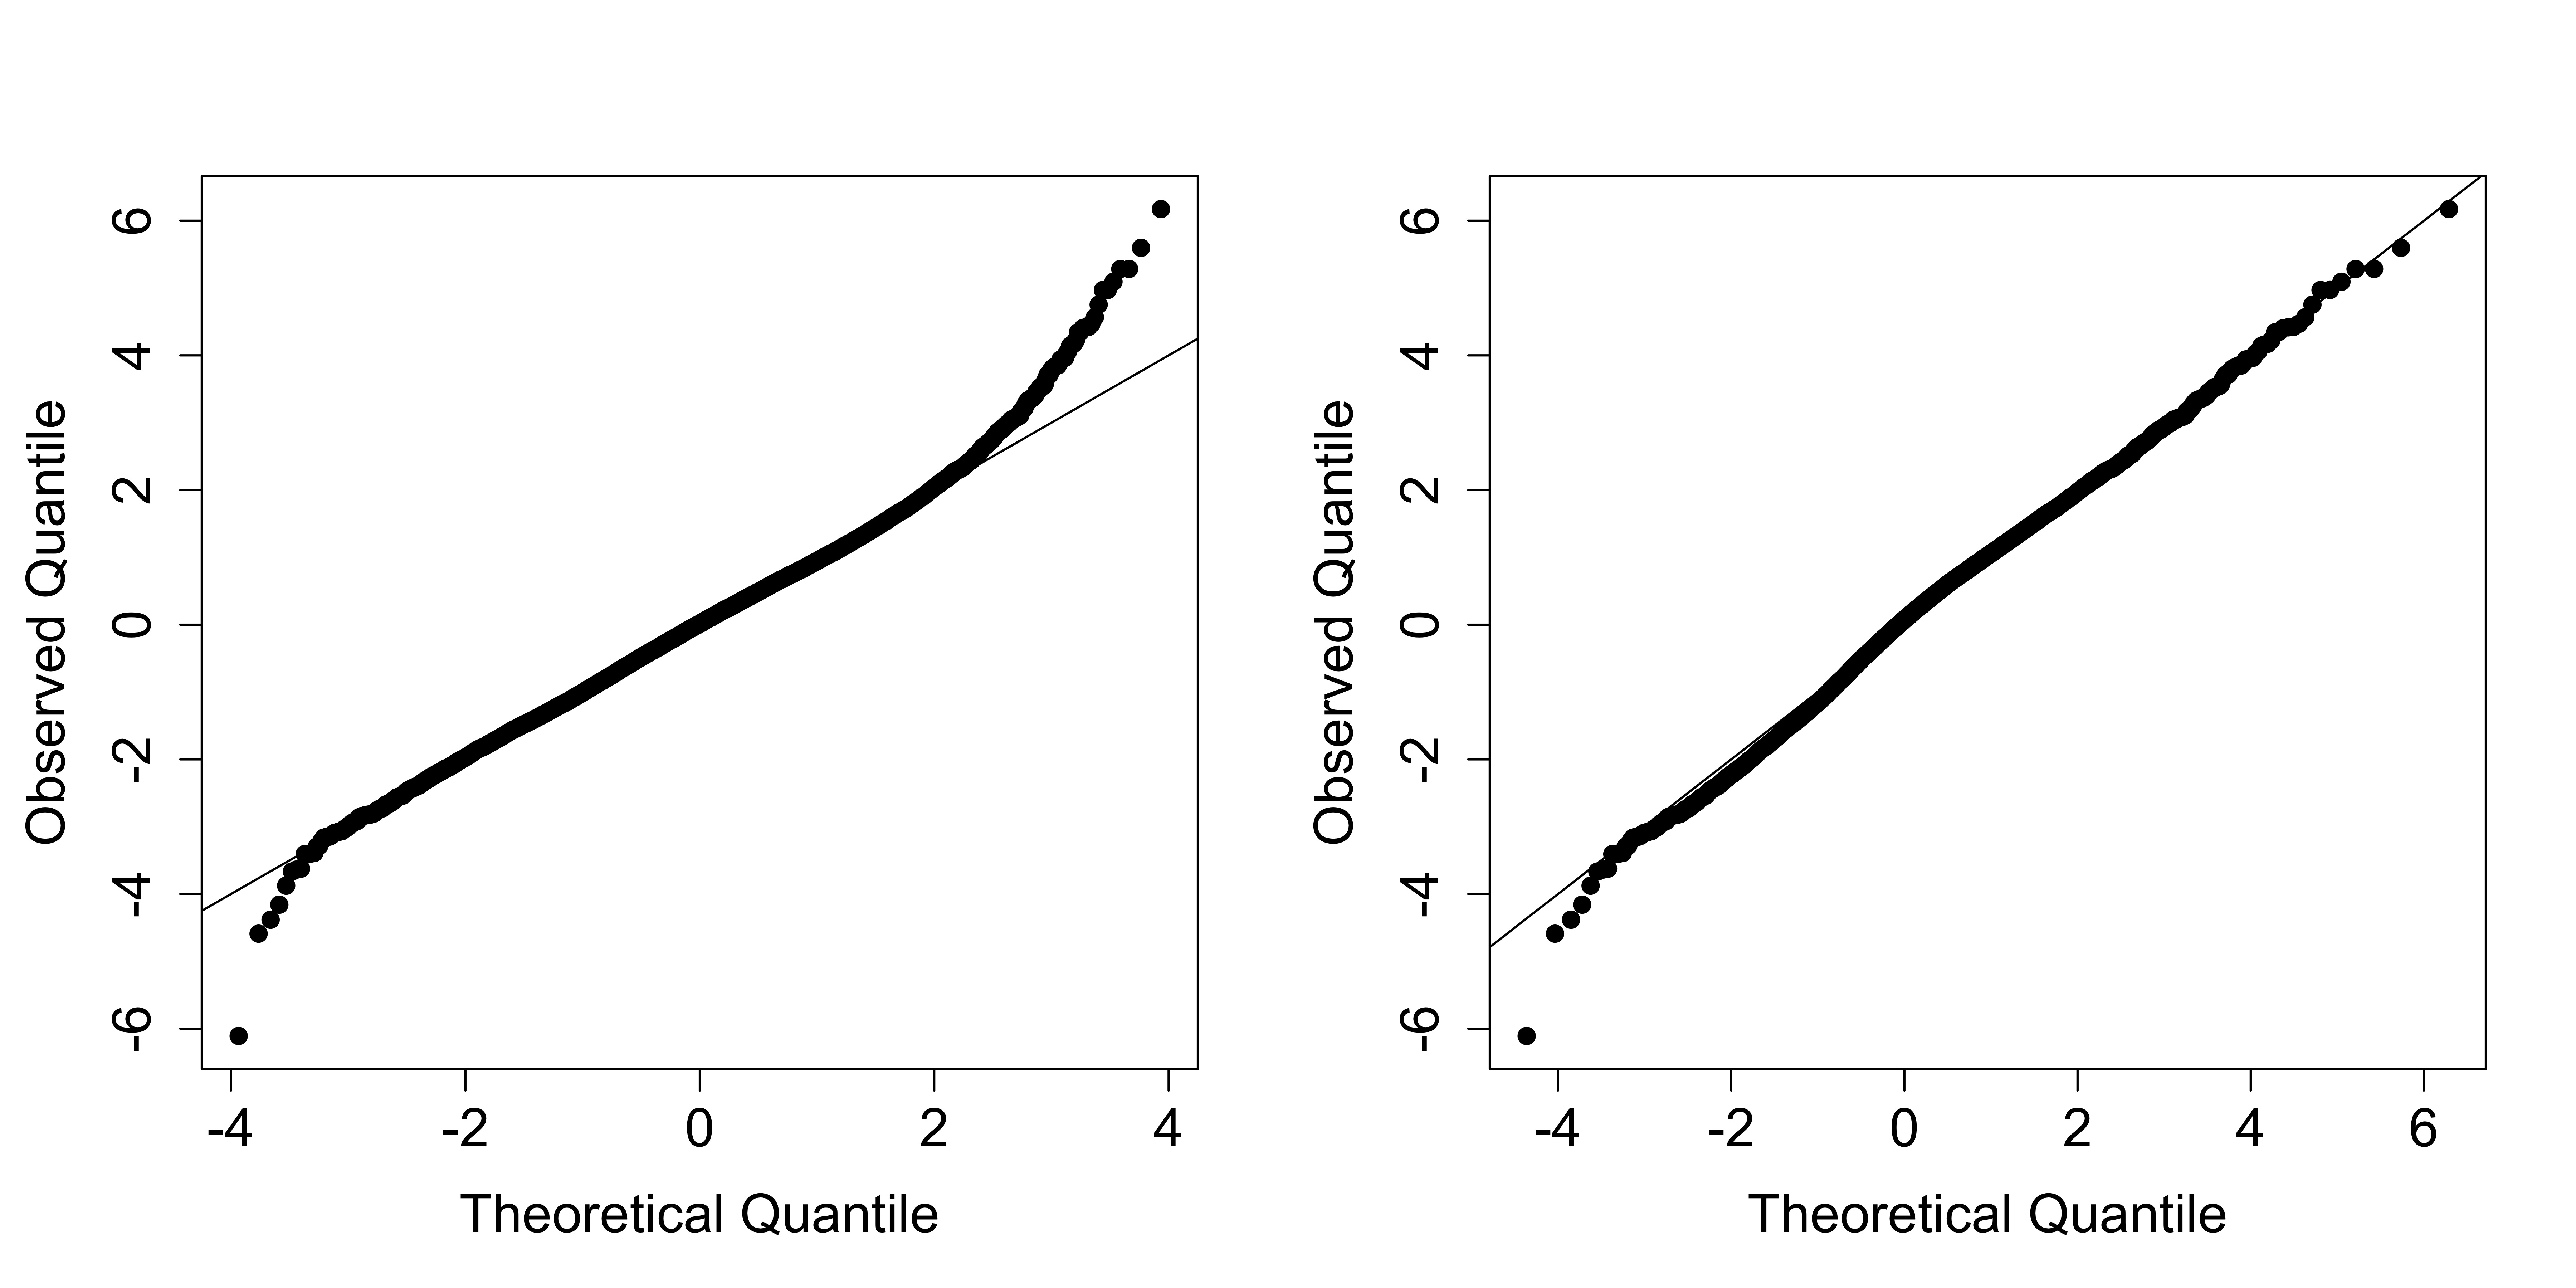
\includegraphics[width=0.9\textheight]{qq-res}

 		Gaussian Q-Q plot (left) and skew-$t$ with $a = 10$ and $\lambda = 1$ Q-Q plot (right)
 	\end{center}
 \end{frame}

 \begin{frame}\frametitle{Cross-validation}
 	\begin{itemize}\setlength\itemsep{\fill}
 	\item We split the sites into training and testing
 	\item We found that $K=15$ knots and censoring at $T$ equal to the median with no time series gave the best results
 	\item Results were not sensitive to these tuning parameters
 	\item This model was 5\% more accurate (Brier score) than GP
 	\item The max-stable model fit was 15\% less accurate than GP
 	\end{itemize}
 \end{frame}

 \begin{frame}\frametitle{Fitted 99$^{th}$ percentile - Gaussian}
 	\begin{center}
 		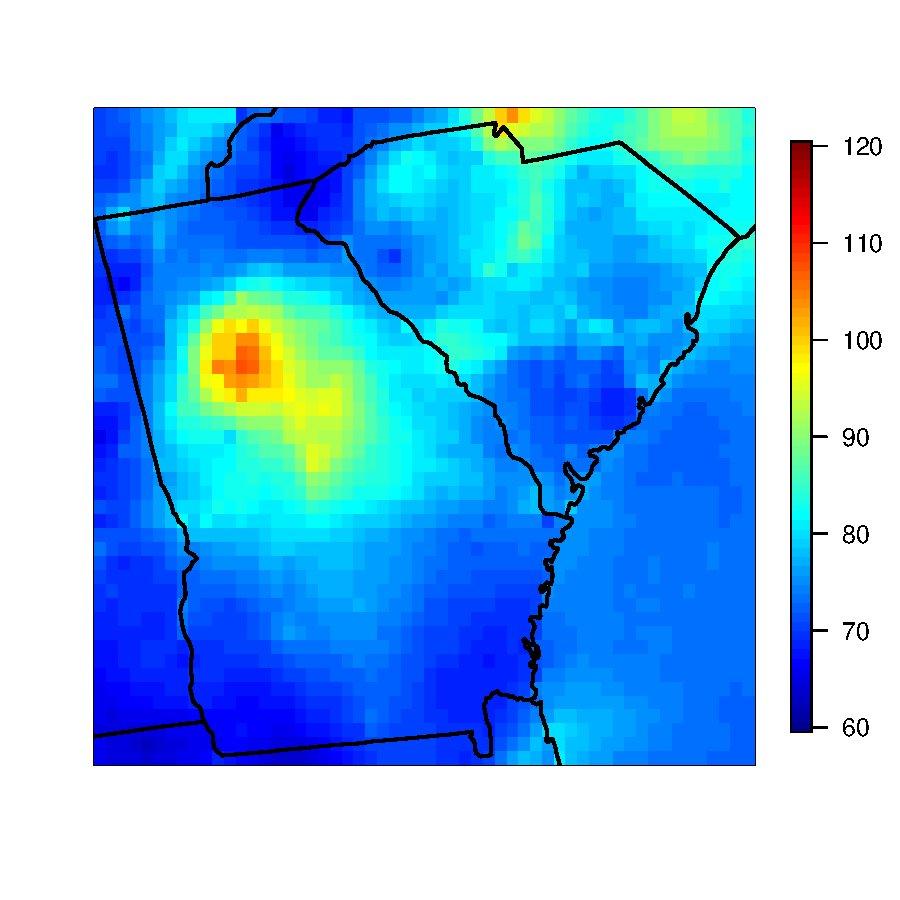
\includegraphics[width=0.45\linewidth]{q99gaus}
 		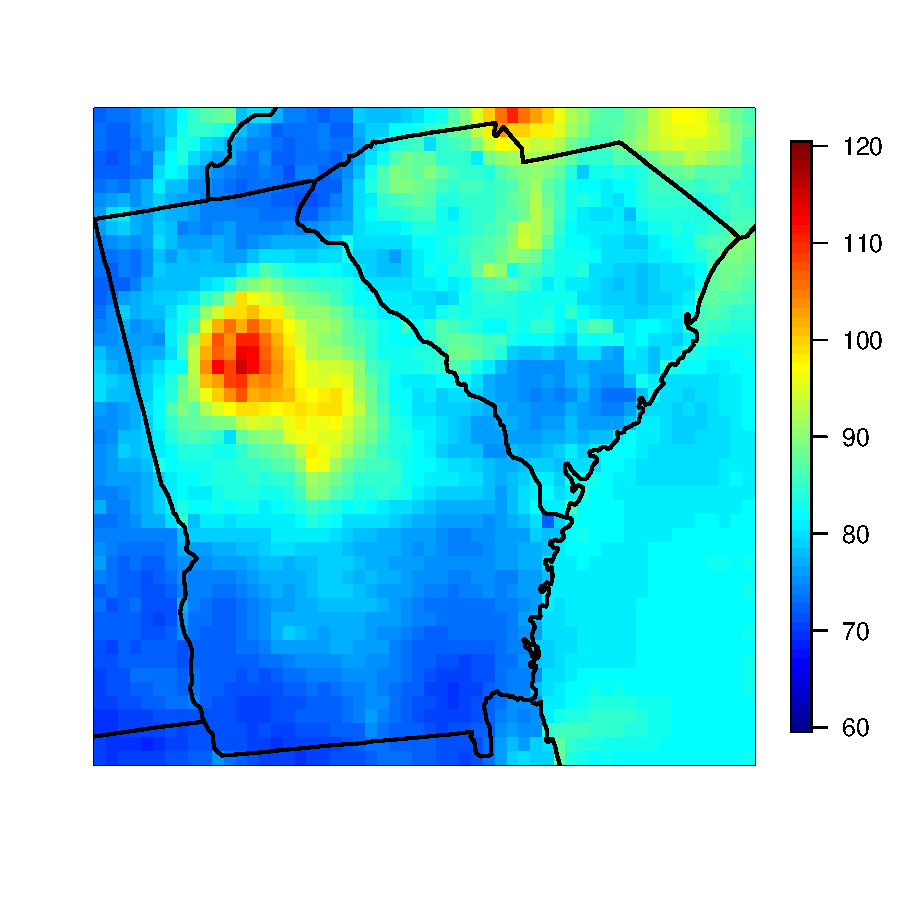
\includegraphics[width=0.45\linewidth]{q99skewtTS}

 		Gaussian (left) Symmetric-$t$, 10 knots, T = 75, Time series (right)
 	\end{center}
 \end{frame}

 \begin{frame}\frametitle{Difference (Thresholded $t$ - Gaussian)}
 	\begin{center}
 		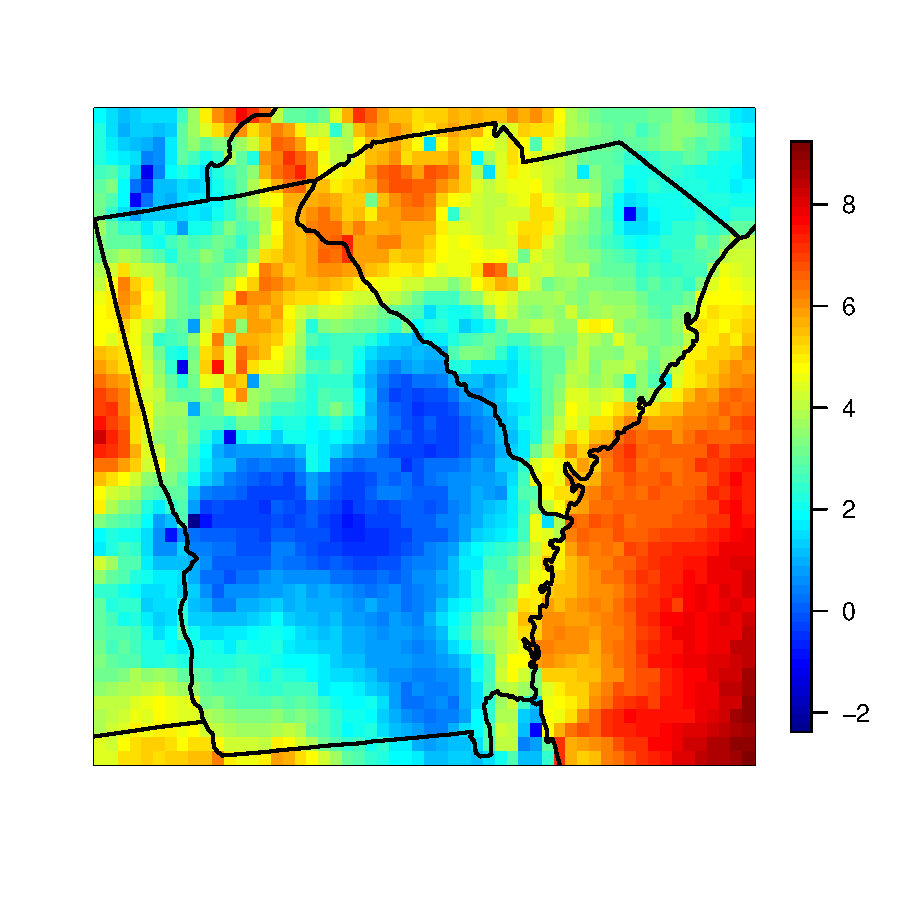
\includegraphics[width=0.55\linewidth]{q99diffgausskewt}

 		Difference between Symmetric-$t$, 10 knots, T = 75 and Gaussian
 	\end{center}
 \end{frame}


\begin{frame}{Questions}
  \begin{itemize} \setlength{\itemsep}{1em}
    \item Questions?
    \item Thank you for your attention.
    \item Acknowledgment: This work was funded by EPA STAR award R835228
  \end{itemize}
\end{frame}
%
%\begin{frame}[allowframebreaks]{References}
%  \begin{itemize} \setlength{\itemsep}{1em}
%    \item Balkema, A. A. and de Haan, L. (1974). Residual life time at great age, {\it Annals of Probability}, {\bf 2}, 792--804.
%    \item de Carvalho, M. and Davison, A. C. (2014). Spectral density ratio models for multivariate extremes, {\it Journal of the American Statistical Association}, {\bf 109}, 764--776.
%    \item Coles, S. G., Heffernan, J., and Tawn, J. A. (1999). Dependence measures for extreme value analysis, {\it Extremes}, {\bf 2}, 339--365.
%    \item Coles S. G. and Tawn, J. A. (1991). Modelling extreme multivariate events. {\it Journal of the Royal Statistical Society: Series B (Methodological)}, {\bf 53}, 337--392.
%    \item Demarta, S. and McNeil, A. J. (2007). The $t$ copula and related copulas. {\it International Statistical Review}, {\bf 73}, 111--129.
%    \item Falk. M., H\"{u}sler, J., and Reiss, R. D. (2010). {\it Laws of Small Numbers: Extremes and Rare Events}. Springer Basel.
%    \item Kim, H.-M., Mallik, B. K., and Holmes, C. C. (2005). Analyzing nonstationary spatial data using piecewise Gaussian processes. {\it Journal of the American Statistical Association}, {\bf 100}, 653--668.
%    \item Gnedenko, B. (1943). Sur la distribution limite du terme maximum d'une s\'{e}rie al\'{e}atoire. {\it Annals of Mathematics}, {\bf 44}, 423--453.
%    \item Gneiting, T. and Raftery, A. (2007). Strictly proper scoring rules, prediction, and estimation. {\it Journal of the American Statistical Association}, {\bf 102}, 359--378.
%    \item Gumbel, E. J. (1960). Multivariate extremal distributions. {\it Bulletin de l'Institut International de Statistique}, {\bf 37}, 471--475
%    \item Huser, R. and Davison, A. C. (2014). Space-time modelling of extreme events. {\it Journal of the Royal Statistical Society: Series B (Statistical Methodology)}, {\bf 76}, 439--461.
%    \item Padoan, S. A. (2011). Multivariate extreme models based on underlying skew-$t$ and skew-normal distributions. {\it Journal of Multivariate Analysis}, {\bf 102}, 977--991.
%    \item Reich, B. J. and Shaby, B. A. (2012). A hierarchical max-stable spatial model for extreme precipitation. {\it Annals of Applied Statistics}, {\bf 6}, 1430--1451.
%    \item Smith R. L. (1990). Max-stable processes and spatial extremes, unpublished manuscript.
%    \item Tawn, J. A. (1990). Modelling multivariate extreme value distributions. {\it Biometrika}, {\bf 77}, 245--253.
%    \item Zhang, H. and El-Shaarawi, A. (2010). On spatial skew-Gaussian processes and applications. {\it Environmetrics}, {\bf 21}, 33--47.
%  \end{itemize}
%\end{frame}

\end{document}